% Chapter 3

\chapter{技术路线及预测结果} 
\label{Chapter3}  
\section{技术路线选取}
基于之前的调研,在实际的预测分析中采取了三种方案进行预测分析:
\begin{itemize}
	\item 基于时间序列分析的Arima分析方法
	\item 多层感知机方法
	\item 时空残差网络方法
\end{itemize}
\section{Arima分析方法}
\subsection{模型概述}
如前文中所提到\ref{arima}, ARIMA模型全称为自回归积分滑动平均模型,主要用于时间序列预测。其主要思想为,将序列转化为平稳序列后,因变量的值由其滞后值与随机误差的现值和滞后值表示\cite{10.1007/978-981-10-8636-6_34}。其数学表达式如下:
\begin{equation}
\left( 1 - \sum _ { i = 1 } ^ { p } \phi _ { i } L ^ { i } \right) ( 1 - L ) ^ { d } X _ { t } = \left( 1 + \sum _ { i = 1 } ^ { q } \theta _ { i } L ^ { i } \right) \varepsilon _ { t }
\end{equation}
其中,$L$ 为滞后算子,$\phi$ 和 $\theta$ 为待求系数,$p$ 为自回归系数, $q$ 为滑动平均阶数,$d$为差分阶数
\subsection{分析过程}
以数据中第 \textbf{840} 号基站网格为中心的9个网格的每小时驻留人数的时序序列进行为例进行分析
\subsubsection*{检测序列是否平稳}
取两周的数据,观察序列的滑动平均与滑动方差(窗口长度为12),可以看到均值在较大范围内变化。进一步对序列差分,均值在很小范围内波动,基本可以视为平稳序列。
\begin{figure}[ht]
\centering
\subfloat[序列滑动平均]{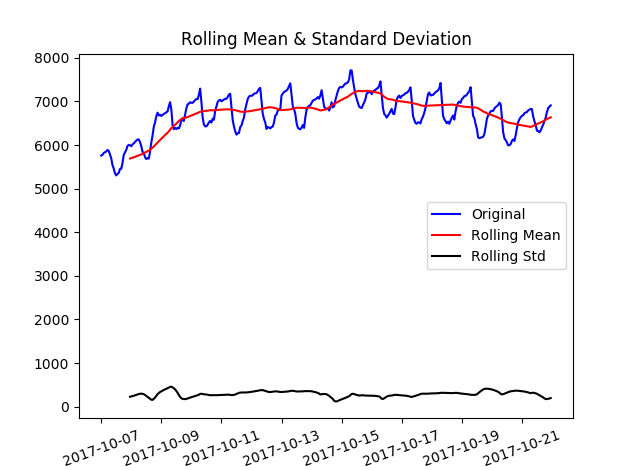
\includegraphics[width=0.50\textwidth]{ARIMA1.png}}
\subfloat[序列滑动方差]{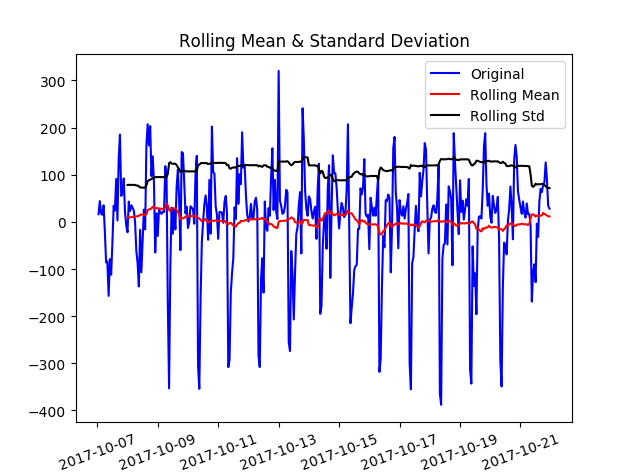
\includegraphics[width=0.50\textwidth]{ARIMA2.png}}
\hfill
\caption{检查序列是否平稳}
\label{fig:ARIMA1}
\end{figure}

\subsubsection*{对序列进行周期性和趋势性分解}
从图(\ref{fig:ARIMA3})中可以看出,数据有长期的变化趋势和明显的周期性变动,并且其残差项接近白噪声。

\begin{figure}[ht]
\centering
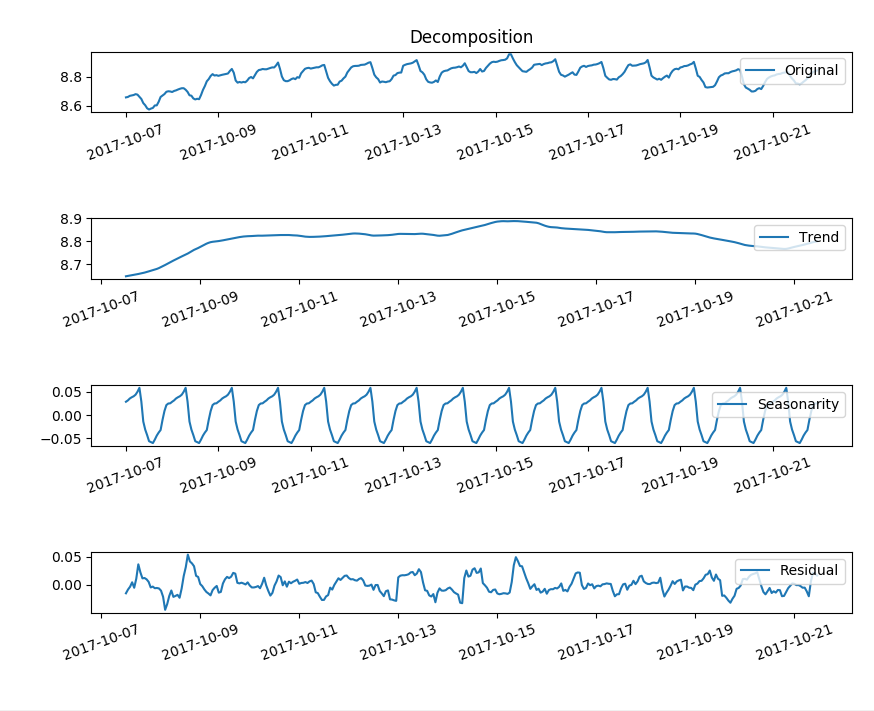
\includegraphics[width=0.8\textwidth]{ARIMA3.png}
\caption{序列周期性和趋势性分解}
\label{fig:ARIMA3}
\end{figure}

\subsubsection*{通过自相关和偏相关函数确定模型阶数}
从图(\ref{fig:ARIMA4})中可以观测出,依据自相关函数第一次降低到误差线以下可以确定MA阶数q=4,偏相关函数第一次降低到误差线以下可以确定AR阶数p=2。

\begin{figure}[ht]
\centering
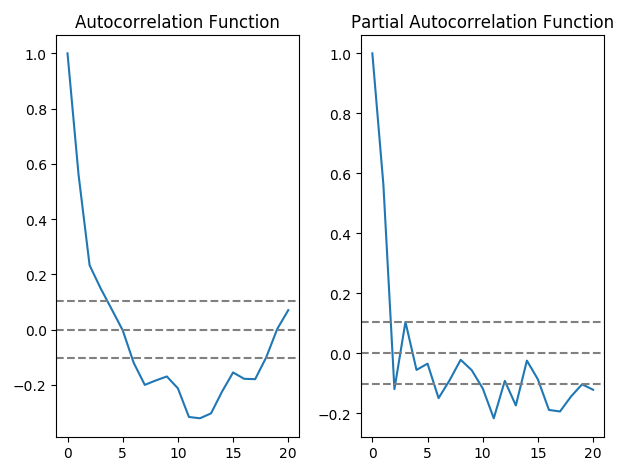
\includegraphics[width=0.8\textwidth]{ARIMA4.png}
\caption{确定模型阶数}
\label{fig:ARIMA4}
\end{figure}
\subsection{预测结果和分析}
最终的预测结果如图(\ref{fig:ARIMA5})所示,可以看出与原始序列对比,预测结果趋势一定程度与真值相近,但是峰值上存在较大误差。
\begin{figure}[ht]
\centering
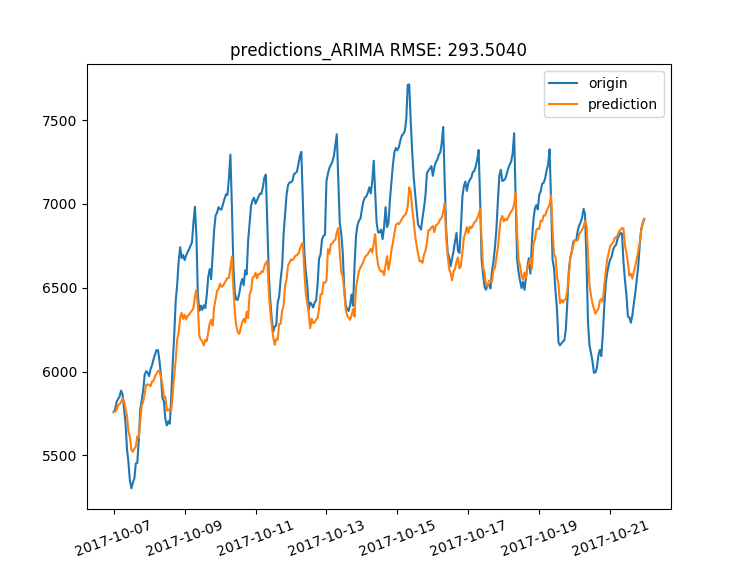
\includegraphics[width=0.8\textwidth]{ARIMA5.png}
\caption{预测结果}
\label{fig:ARIMA5}
\end{figure}
可以认为
\begin{enumerate}
	\item 利用Arima模型对本项目的数据进行建模可以预测趋势但是存在一定误差
	\item 可能的原因是序列的相关性是跳跃的,即某时刻的数据可能与1小时前、2两小时前、24小时前、48小时前、一周前的数据等相关性更高,而不是与之前的数据随时间间隔增大相关性逐渐降低
	\item 另外Arima模型所能考虑的空间上的范围也是有限的,其必然会导致预测精度上的误差
	\item 对于之后的模型建立,就需要考量时间相关性的构成和选取乃至对于空间上短程和长程相互影响的处理方法
\end{enumerate}


\section{时空残差网络方法}
\subsection{理论基础}
对于信令数据可以采取一下两种向量化方法:
\begin{equation}
\begin{split}
p = & f(id,time,week[weather,air condition,...])\\
p = & f(id,time,week,p(last hour),p(yesterday),p(last week),p(last month))
\end{split}
\end{equation}
其中,p 代表人口数据,可以通过维度的不同进行不同的表达(一维表示驻留人数,三维表示驻留人数,出发人数和到达人数),特别的,id 中隐含了地域的信息。
\subsection{分析手段}
采用有监督人工神经网络,期望输出为驻留人数、出发人数、到达人数,其基本架构如图(\ref{fig:3.1})所示。
\begin{figure}[ht]
\centering
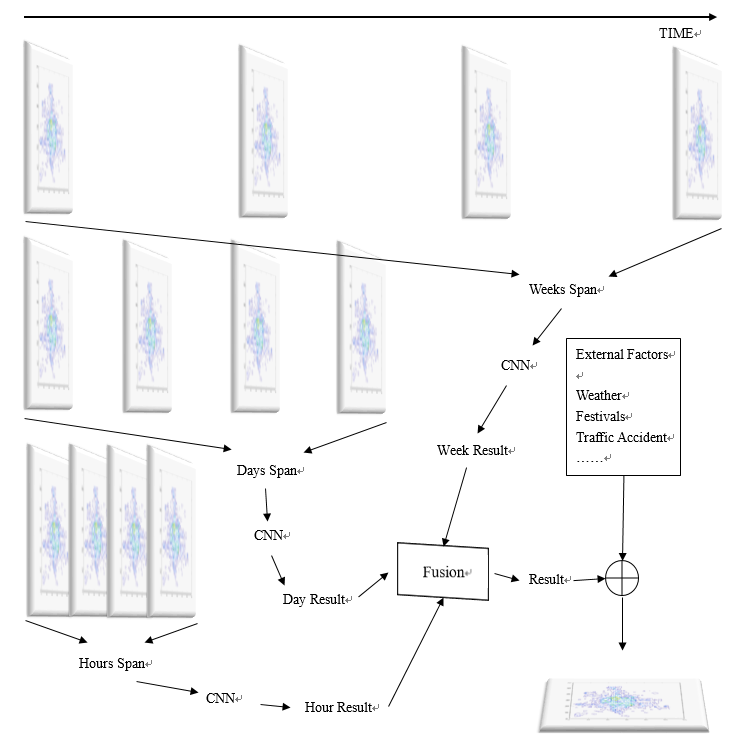
\includegraphics[width=0.8\textwidth]{ournet.png}
\caption{网络搭建基本构型}
\label{fig:3.1}
\end{figure}
输入为数据的特征,人工选取:我们认为主要以人数与 星期几(已有)、具体小时(已有)、位置(已有)、天气(可以爬取)、前一小时的人数(对已有数据处理)等主要因素有关。
同时我们以获得数据中的驻留人数、出发人数、到达人数作为标签,期望输出。
利用期望输出与网络输出之间的误差建立学习信号反向传播,修正网络权重。
\subsubsection*{初步网络搭建}
中间两个隐层,每个隐层20个神经元,采取全连接。
虽然说基站数量为2265个,我们的网络权重大约是600个待定参数好像不太够保存所有基站的信息。但是,注意到我们关注的是一片区域的总人口数据,而不是特指
某个基站的总人口个数,所以我们的网络只要区分出这种大概有同一人口特性的区域即可,最终对人口驻留,流动的分析也是基于区域进行分析的,所以600个左右的待定参数是够用的。
\subsubsection*{两种可能方案}
\begin{itemize}
	\item 方案A:多输入多输出(针对所有点的神经网络模型)\\
	类似于图片处理,2265个基站,输入即为2265*n,其中n为输入特征(星期,小时,ID(位置特征)等),输出为2265*3,3为标签个数(驻留人数、出发人数、到达人数)
	\item 方案B:少输入少输出(针对某一点的神经网络模型)\\
	针对某一个基站或者某一块区域进行训练。输入为特征个数(星期,小时,ID等),输出为3,即驻留人数、出发人数、到达人数。\\
	训练出来的模型是针对某一个基站或者某一块区域(9个基站左右,表示$9km^2$的一个区域)的人口情况。做分析时候要训练多点得到一个区域的数据进行分析。\\
	统计关心区域的总人口驻留,总人口流出,总人口流入来表示这个区域的人口数据。因为守恒关系,一个区域内所有点的人口驻留人数代数和即为该区域的总人口驻留人数,总人口流入与总人口流之差,即为该区域的总人口流入或总人口流出。
\end{itemize}


\subsection{方案设计}
最终的模型基于上述的 ARIMA 的初步分析和多层感知机的结果分析,参考文献中的方法,最终独立搭建了时空残差网络的模型方法。
\subsubsection*{问题建立}
对于人口数据,直观的显示是如图(\ref{fig:map})中显示的按照地图进行划分,而在我们的模型研究中,将其划分为沿着经纬线划分的$M \times N$矩形网格(见图\ref{fig:cluster})
\begin{figure}[ht]
\centering
\subfloat[基于地理信息地图的人流]{\label{fig:map}{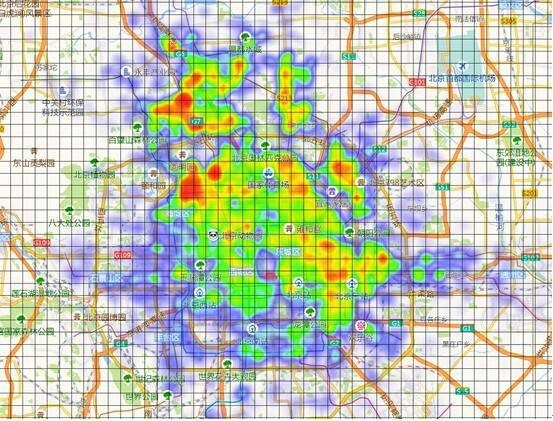
\includegraphics[width=0.45\textwidth]{map.jpg}}}
\subfloat[人流热力矩阵]{\label{fig:cluster}{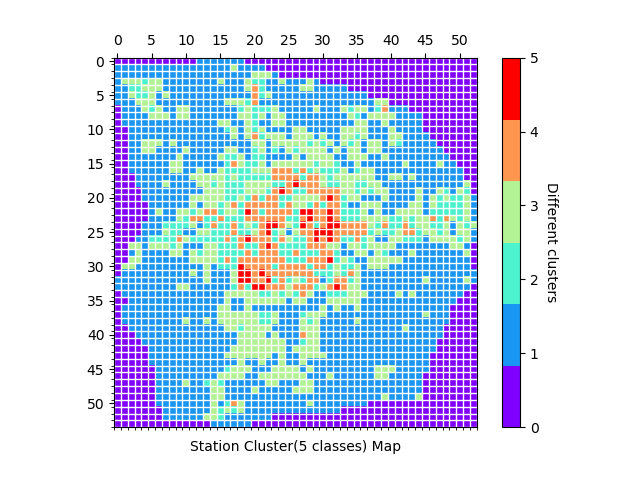
\includegraphics[width=0.45\textwidth]{clusters.png}}}
\hfill
\caption{北京人口区域划分:地理信息地图和人流热力图}
%\label{fig:subfigures}
\end{figure}
\subsubsection*{模型划分}
此问题实际上是想要基于过去的给定观测值进行未来的值的预测的一个回归分析的问题,其数学表达式为:
\\
给定 $\{X_t | t = 0,\cdots,n-1 \}$,预测 $X_{n},\cdots,X_{n+m}$
\subsubsection*{模型理论基础}
模型采用的深度残差网络相比传统的卷积神经网络可以有着更深的结构层数\cite{he2016deep},而实践证明其在图像分类、物体识别等问题中有着相当好的应用效果\cite{he2016identity},所以我们基于这样的网络结构进行模型的搭建。\\
一般地,在残差网络中可以将回归预测模型的问题定义为:
\begin{equation}
X^{(l+1)} = X^{(l)} + \mathcal{F}(X^{(l)})
\end{equation}
其中,$X^{(l+1)}$和$X^{(l)}$分别是第$l$个残差单元的输入和输出,而$\mathcal{F}$为残差函数,而实际上网络的目标就是基于输入值寻找到合适的残差函数,一个典型的残差单元的示意如图(\ref{fig:resident})所示。
\begin{figure}[ht]
\centering
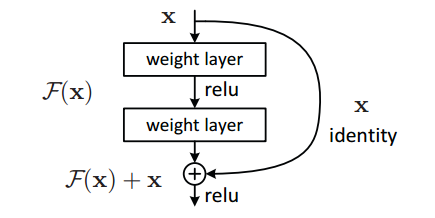
\includegraphics[width=0.8\textwidth]{resident.png}
\caption{残差单元示意图\cite{he2016deep}}
\label{fig:resident}
\end{figure}
\subsubsection*{残差网络结构}
前文的图(\ref{fig:3.1})很好地展示了本研究所采用的残差网络的架构,在时间周期层面上考虑 \textbf{小时、天、周}三个不同层次的影响,并利用卷积考虑空间上的相互关联,最后再加入外部因素的影响。 模型分别采取预测时刻的最近三个小时、一天前的四个小时和一周前的两个小时的数据作为输入,在网络中得到不同的权重,再计算残差实现反向传播。\\
\indent 在实际的网络设计中,考虑到城市不同区域之间的相互关联(如依靠地面公路、地铁的流动)进行卷积核的大小的调整和对于激活函数的定义。
\subsubsection*{数据混合}
模型中的三个不同时间周期的数据可以用参数矩阵的方法进行混合:
\begin{equation}
\mathbf { X } _ { R e s } = \mathbf { W } _ { hour } \circ \mathbf { X } _ { hour }  + \mathbf { W } _ {day } \circ \mathbf { X } _ { day }  + \mathbf { W } _ { week } \circ \mathbf { X } _ { week } 
\end{equation}
其中的乘法为矩阵乘法(哈达马积),而参数$W_{hour}$,$W_{day}$和$W_{week}$为模型参数
\subsubsection*{模型算法和优化方法}
模型的算法步骤和优化方法见算法框图(\ref{al}) 
\begin{algorithm}[t]
\caption{ResNet Training Algorithm} %算法的名字
We first construct the training
instances from the original sequence data.\\ Then, RenNet is trained via backprogagation and Adadelta.\\
\hspace*{0.02in} {\bf Input:} %算法的输入, \hspace*{0.02in}用来控制位置,同时利用 \\ 进行换行
Historical observations: \{ $X_0,\cdots,X_{n-1}$ \}\\
\hspace*{0.02in} Lengths of closeness, period, trend sequences: $l_c$,$l_p$,$l_q$\\
\hspace*{0.02in} Period, trend span: q\\
\hspace*{0.02in} {\bf Output:} %算法的结果输出
learnt ResNet model\\
\begin{algorithmic}[1]
\State \#construct training instances\\
D <- None % \State 后写一般语句
\For{t in all available time interval [1,n-1]} % For 语句,需要和EndFor对应
  \State $S_c = [X_{t-l_c},X_{t-(l_c-1)},\cdots,X_{t-1}]$
	\State $S_p = [X_{t-l_p*p},X_{t-(l_p-1)*p},\cdots,X_{t-p}]$
	\State $S_q = [X_{t-l_q*q},X_{t-(l_q-1)*q},\cdots,X_{t-q}]$\\
Put an training instance ($\{S_c,S_p,S_q \},X_t$) into D
\EndFor
\# define the loss
\\
LOSS = MSE($X_t$,output of ResNet)\\
\# train the model\\
\# initialize all learnable parameters cita in ResNet\\
Epoch <- int(numbers)

\For{epoch in range(Epoch)} % For 语句,需要和EndFor对应
  \State \textbf{Repeat}
	\State Select an instance $D_b$ from D
	\State $\theta$ by minimizing the LOSS with $D_b$
\textbf{Until} all elements of D used\\
\# save model every 10 epoches
  \If{epoch \% 10 == 0} % If 语句,需要和EndIf对应
    \State Save model
  \EndIf
\EndFor
\end{algorithmic}
\label{al}
\end{algorithm}